\section{Contexte}
L'association Baleinev organise, depuis plus de 25 ans, le festival de musique “Baleinev Festival” sur le campus de la HEIG-VD et aime se démarquer par son originalité.

En 2014, le festival proposait pour la première fois “Pimp My Wall”, un concept qui consiste à utiliser des fenêtres orientées sur la cour comme écrans géants, affichant du contenu interactif, des animations visuelles et la possibilité de dessiner à distance.

\begin{figure}[H]
  \centering
  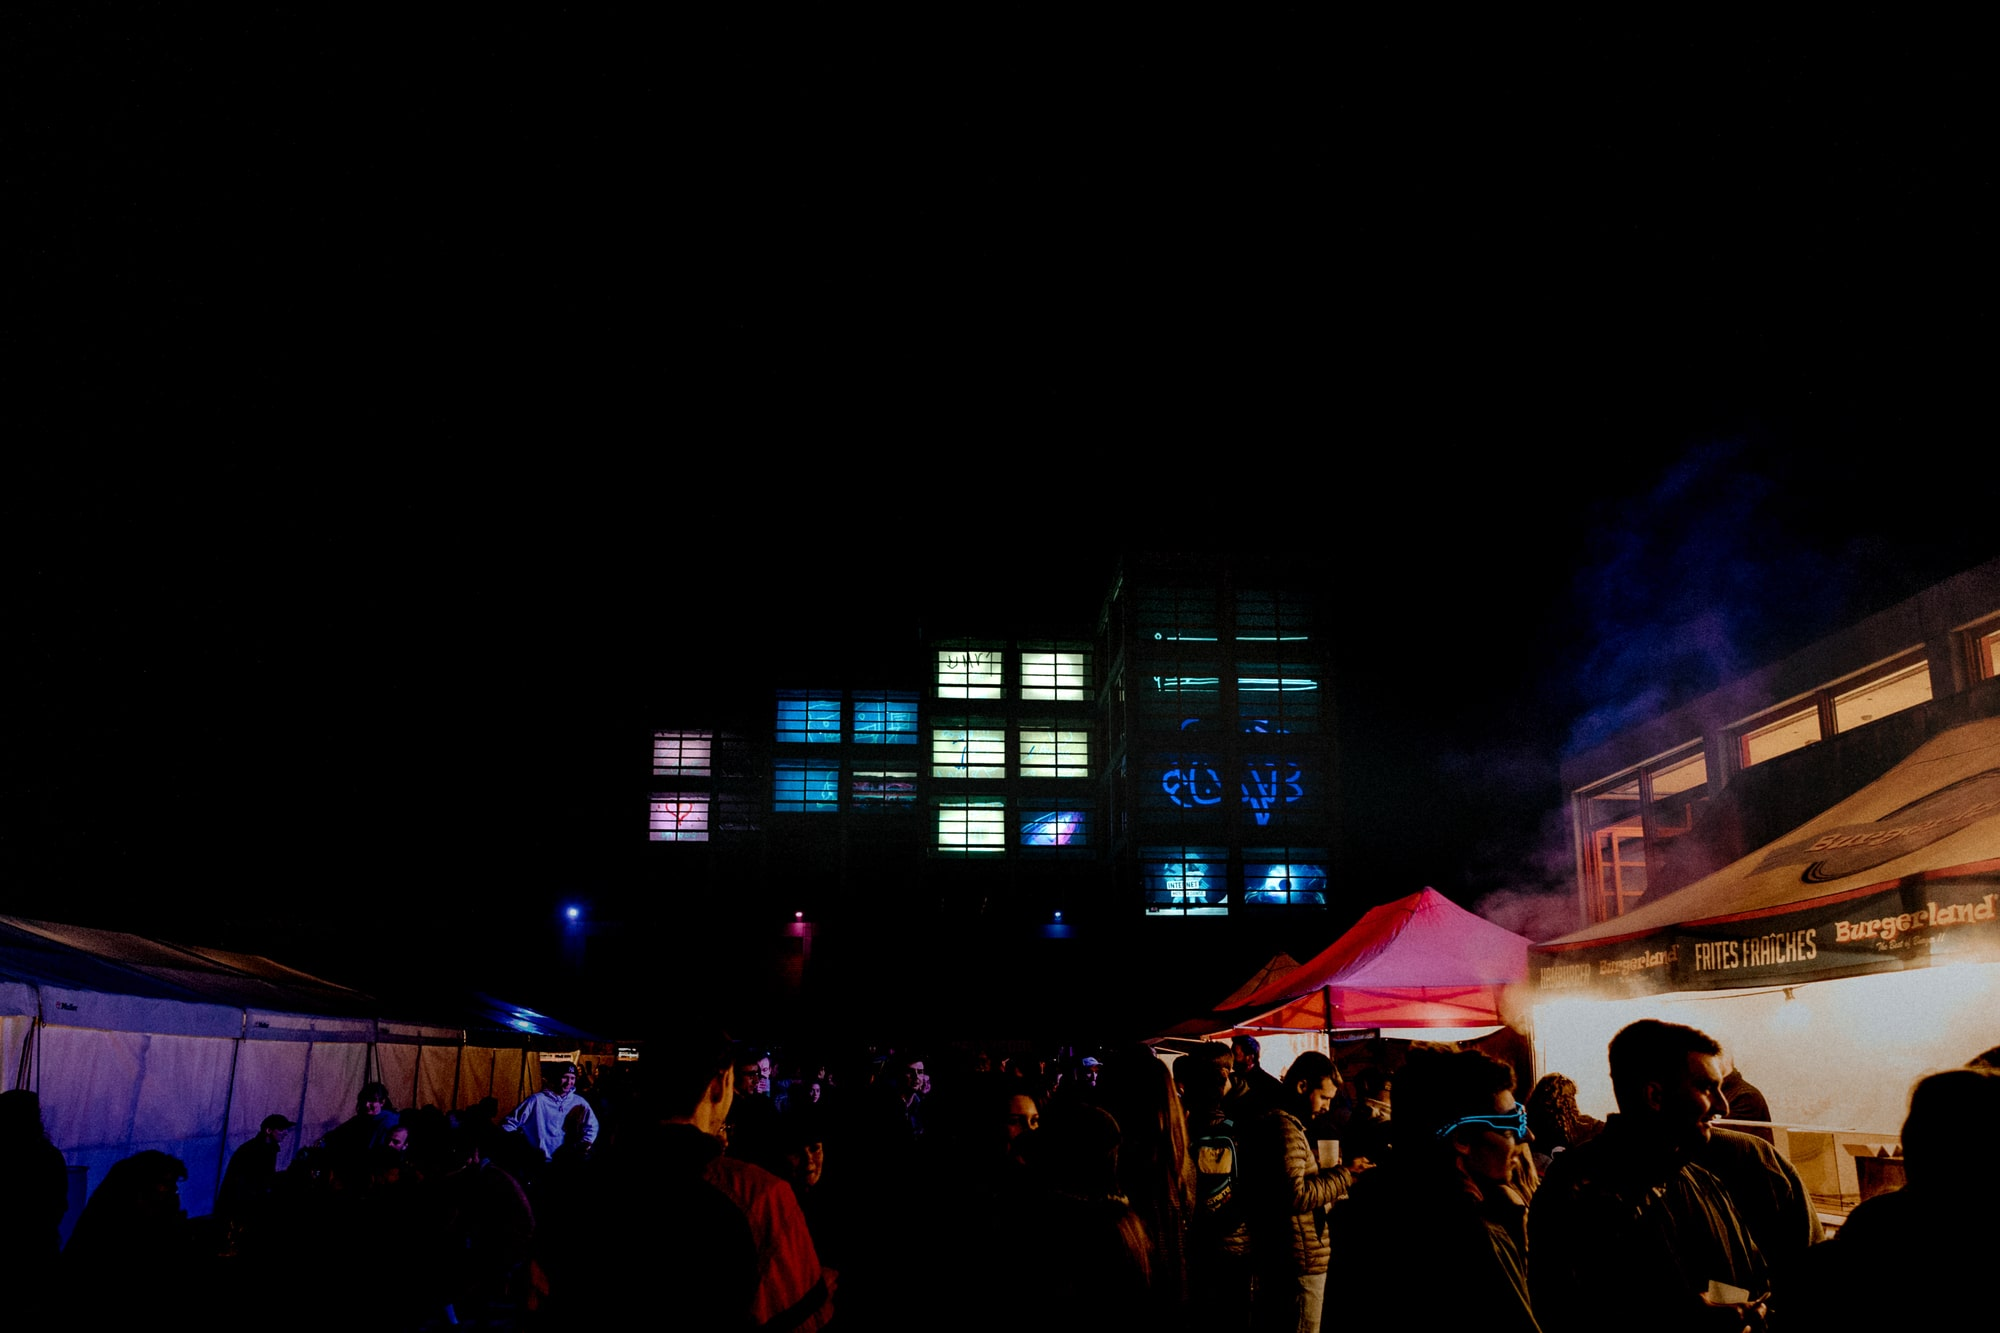
\includegraphics[width=0.8\textwidth]{assets/figures/pmw-ak.jpg}
  \begin{center}
    \textit{Photo réalisée par Antoine Kaelin}
  \end{center}
  \caption{Écrans de Pimp My Wall lors du Baleinev Festival 2023}
  \label{fig:pmw-baleinev-2023}
\end{figure}

En 2018, le concept a été repris à partir de zéro et a donné naissance à \gls{beescreens}, la nouvelle version open source aux technologies modernes. L'ambition de cette nouvelle version est de proposer une collection d'applications interactives pouvant sortir du cadre du Baleinev Festival. De plus, l'ajout est la gestion d'une nouvelle application se veut le plus aisé possible, permettant ainsi à de nouveaux développeurs de pouvoir rapidement créer et déployer une nouvelle application.

C'est dans ce contexte qu'est né le projet de ce travail de Bachelor avec la volonté de créer une nouvelle application interactive à projeter entre autres sur un sous-ensemble des écrans du festival.

\section{Présentation r/place}
\gls{reddit} (\href{https://www.reddit.com}{reddit.com}), sûrement le forum en ligne le plus connu au monde, a l'habitude de faire des expériences pour le premier avril. En 2017, \gls{reddit} présente pour la première fois leur concept r/place.

r/place~\cite{rplace} offre une toile géante virtuelle permettant à tout le monde de placer un pixel d'une couleur choisie parmi une liste prédéfinie. Chaque personne doit attendre un certain temps (5 minutes) avant de reposer un nouveau pixel. Cela oblige une collaboration des utilisateurs afin de réaliser des dessins de qualité, ce qui implique qu'aucun individu ou groupe ne peut nuire trop fortement à l'ensemble de l'\oe{}uvre.

En 2022, une nouvelle version du r/place est mise en place et plus de 6 millions de personnes participent à cette édition. La toile est agrandie pour atteindre des dimensions de 2000x2000 pixels et celle-ci se trouve remplie de créations en tout genre réalisées par diverses communautés pendant plusieurs jours (voir figure \ref{fig:rplace2022}).

\begin{figure}[H]
  \centering
  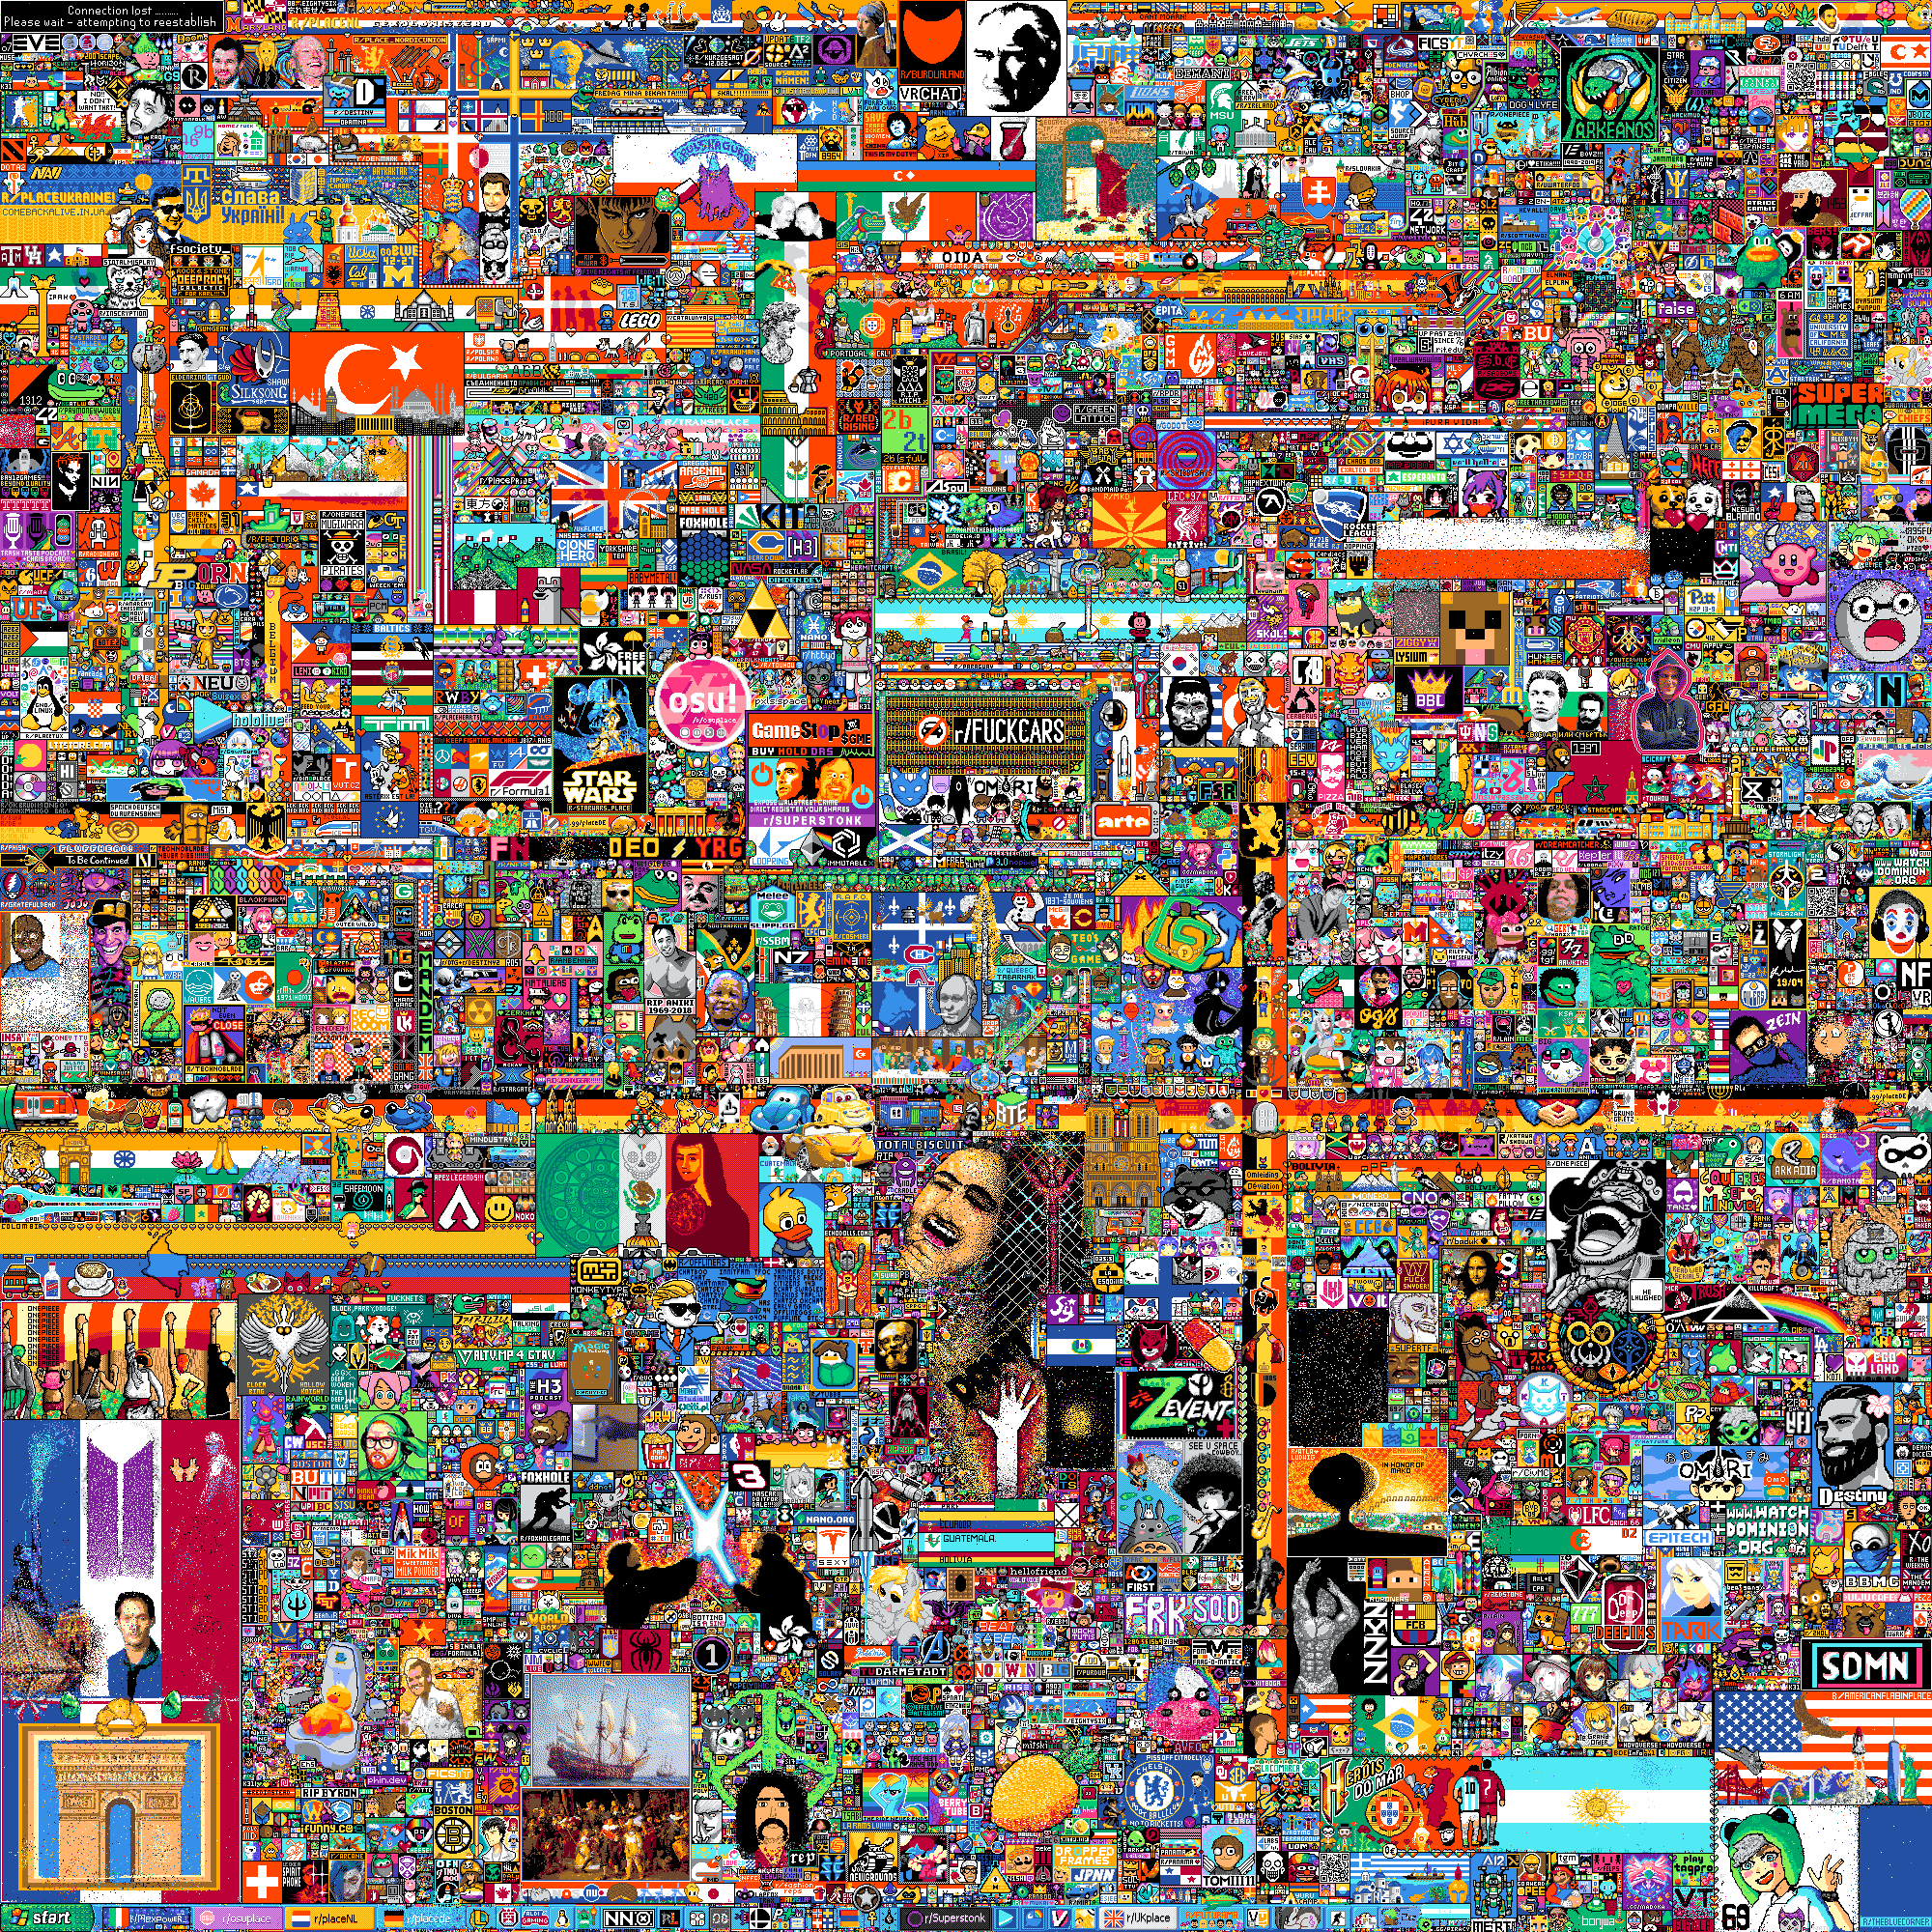
\includegraphics[width=0.8\textwidth]{./assets/figures/rplace.png}
  \caption{Résultat du r/place de 2022}
  \label{fig:rplace2022}
\end{figure}

Les codes sources de ces deux événements ne sont malheureusement pas disponibles. Cependant, les ingénieurs du r/place ont publié des articles présentant leur architecture et leur implémentation. Ces articles sont disponibles sur le site de \gls{reddit}~\cite{rplace2017, rplace2022}. Ces articles seront utilisés comme référence pour ce travail de Bachelor mais l'architecture ainsi que l'implémentation seront complètement différentes. En effet, le but est de créer seul une version open source de r/place. L'envergure du projet ainsi que la taille du public visé sont évidemment bien moindres que celles du r/place original.

\section{Cahier des charges}
\label{sec:cdc}

\subsection{Objectifs}
\label{sec:objectifs}

Le but principal de ce travail de Bachelor consiste à recréer une version open source du fameux r/place de \gls{reddit}. Cette variante sera nommée \gls{beeplace} afin de s'aligner avec le nom de l'écosystème \gls{beescreens}.
Cette application, comme le r/place original, a comme objectif de permettre aux utilisateurs de poser des pixels sur une toile virtuelle partagée entre tous. Chaque utilisateur pourra poser un ou plusieurs pixels d'une couleur choisie parmi une liste prédéfinie. Afin de maximiser la collaboration entre les utilisateurs et minimiser les dégâts causés par des utilisateurs malintentionnés, ceux-ci devront attendre un certain délai entre chaque pose de pixel.

En effet, le concept \gls{beeplace} se base sur les conclusions réalisées à propos de l'application existante, Pimp My Wall. La problématique est la suivante: Pimp My Wall est une application trop permissive. Les utilisateurs peuvent dessiner de manière entièrement libre sur la toile virtuelle et cela engendre des comportements inappropriés. Le public cible, les personnes présentes au Baleinev Festival, est relativement jeune et l'ambiance festive de la soirée amène plus facilement à des dérives. Comme les créations des festivaliers sont affichées en temps réel sur les murs de l'école, il est nécessaire de modérer les créations des utilisateurs. Cette modération est fastidieuse, peu gratifiante et demande beaucoup de temps.

Afin de pallier à ce problème, l'idée de \gls{beeplace} est née. En imposant un délai entre la pose de pixels aux utilisateurs, ceux-ci seront moins enclins à réaliser des créations inadaptées car cela leur demanderait un effort plus conséquent. Dans le cas où des débordements auraient quand même lieu, la modération pourrait remettre à zéro une zone de la toile en quelques clics. Ce qui ferait perdre énormément de temps aux usagers problématiques et les dissuaderait de recommencer.


En plus de l'application en elle-même, des critères non-fonctionnels sont à prendre en compte. Tout d'abord, il est nécessaire d'assurer sa montée en charge afin qu'elle puisse supporter des possibles hausses de fréquentation, notamment le soir du festival. Ce critère sera vérifié grâce à des tests prévus à cet effet. De plus, il est important d'assurer l'intégration continue de l'application au sein de l'écosystème \gls{beescreens}. En effet, \gls{beeplace} fera partie intégrante de l'écosystème existant et devra donc être correctement intégrée afin de pouvoir être facilement utilisée dans le futur. Pour finir, l'application doit être agréable d'utilisation sur téléphone car les utilisateurs du festival utiliseront principalement ce moyen d'interaction.

\subsection{Fonctionnalités}

Afin d'avoir une idée plus précise des tâches à réaliser, les diverses fonctionnalités de l'application ont été listées. Celles-ci sont catégorisées selon leur importance. Les fonctionnalités \textbf{required} sont nécessaires au bon fonctionnement de l'application. Les \textbf{essential} aident beaucoup à la qualité du projet final et pour finir les \textbf{nice-to-have} améliorent surtout l'expérience utilisateur des usagers ainsi que des administrateurs qui ont la tâche de supprimer les éventuels débordements.

\subsubsection{Fonctionnalités \guillemotleft required\guillemotright}

\begin{itemize}
  \item L'utilisateur arrive sur une page affichant la toile virtuelle au complet.
  \item La toile s'actualise avec les modifications réalisées par les autres utilisateurs.
  \item L'utilisateur peut zoomer ou dézoomer sur la toile afin de voir les moindres détails.
  \item L'utilisateur voit facilement le nombre de pixels qu'il a actuellement la possibilité de placer sur la toile.
  \item L'utilisateur peut sélectionner un pixel, choisir une couleur parmi plusieurs proposées et le colorier.
  \item Les dimensions de la toile doivent être configurables par un administrateur.
  \item L'utilisateur dispose d'un moyen de recharger ses pixels à placer une fois ceux-ci écoulés. Il peut par exemple recevoir un nombre de pixels définis après un temps d'attente également choisi.
\end{itemize}

\subsubsection{Fonctionnalités \guillemotleft essential\guillemotright}

\begin{itemize}
  \item Il doit être possible, pour un administrateur, de passer la toile dans un mode “lecture uniquement” pour tous les utilisateurs.
  \item Créer des tests de montée en charge de l'application afin d'assurer un bon fonctionnement lors des festivals notamment.
  \item Afin d'éviter que les utilisateurs puissent recharger la page pour recevoir à nouveau des pixels, trouver un moyen de les identifier.
  \item Les coordonnées du pixel sélectionné par l'utilisateur lui sont affichées ainsi que son niveau de zoom.
  \item Créer des tests unitaires ainsi que des tests d'intégration pour s'assurer de la qualité de l'application.
  \item Un administrateur peut choisir une zone à censurer (recouvrir/suppression de pixels d'une couleur) à partir d'un call API en cas de comportement non désiré.
\end{itemize}

\subsubsection{Fonctionnalités \guillemotleft nice-to-have\guillemotright}

\begin{itemize}
  \item Ajouter une interface utilisateur permettant aux administrateurs de censurer plus facilement une zone de la toile via le dashboard.
  \item Une fois ses pixels épuisés, l'utilisateur peut les recharger via un moyen physique.
  \item Faire en sorte que les couleurs disponibles aux utilisateurs soient facilement customisables par l'administrateur (ex: via le dashboard).
  \item Les administrateurs peuvent interdire la pose de pixels à des utilisateurs ou des régions spécifiques.
  \item Les administrateurs peuvent changer la taille de la toile dynamiquement (ex : via le dashboard).
  \item Afficher à chaque utilisateur le nombre de festivaliers actuellement connectés sur la toile.
  \item Développer un mode “affichage”, permettant d'afficher régulièrement un code QR pour rejoindre la toile virtuelle. En plus de ce code QR, ajouter des éléments sollicitant l'interaction de l'utilisateur à la manière d'un économiseur d'écran (ex: des pixels qui s'animent de façon indépendante). Ce mode s'enlèverait automatiquement dès qu'un utilisateur est actif sur l'application.
  \item Ajouter la possibilité de sauvegarder le dessin.
  \item Intégrer la notion de CRDTs (Conflict-free Replicated Data Type), une structure de données permettant d'éviter les conflits notamment dans les systèmes distribués collaboratifs multi utilisateurs.
\end{itemize}

\subsection{Calendrier}

Le projet est séparé en différentes milestones, les dates de celles-ci sont adaptées en fonction des événements clés du semestre, comme les délais de rendu ainsi que le Baleinev Festival 2023 en lui-même.

\subsubsection{Milestone 1 - semaine du 20 au 26 mars}

\begin{enumerate}
  \item Rédaction du cahier des charges
  \item Rédaction de la partie du rapport concernant l'intégration dans l'environnement \gls{beescreens}
\end{enumerate}

\subsubsection{Milestone 2 - semaine du 17 au 23 avril}

\begin{enumerate}
  \item Intégration à l'environnement \gls{beescreens} de l'application \gls{beeplace}
  \item Réalisation d'une première version de l'application afin d'être potentiellement utilisée lors du Baleinev Festival de cette année
\end{enumerate}

\subsubsection{Milestone 3 - semaine du 22 au 28 mai}
\label{milestone3}

\begin{enumerate}
  \item Rédaction du rapport intermédiaire
  \item Utilisation d'outils de tests de montée en charge afin d'identifier les problèmes du code actuel
\end{enumerate}

\subsubsection{Milestone 4 - semaine du 12 au 18 juin}

\begin{enumerate}
  \item Optimisation de l'application afin d'améliorer sa scalabilité
  \item Potentiels tests avec les CRDTs (Conflict-free Replicated Data Type)
\end{enumerate}

\subsubsection{Milestone 5 - semaine du 24 au 30 juillet}

\begin{enumerate}
  \item Réalisation des derniers livrables: le résumé publiable ainsi que le poster
  \item Finalisation du rapport
  \item Implémentation de fonctionnalités “nice-to-have”
\end{enumerate}

Le travail se termine le jeudi 27 juillet avec la remise du rapport et des autres livrables indiqués ci-dessous. La défense du travail aura lieu dans les semaines qui suivent.

\subsection{Livrables}

Les livrables à réaliser pour ce travail de Bachelor sont les suivants:

\begin{itemize}
  \item L'application BeePlace;
  \item Un rapport intermédiaire;
  \item Un rapport final;
  \item Un résumé publiable;
  \item Un poster.
\end{itemize}

